\section{Introduction}
\begin{figure}[t!]
  \centering
  \begin{minipage}[t]{0.49\textwidth}
    \centering
    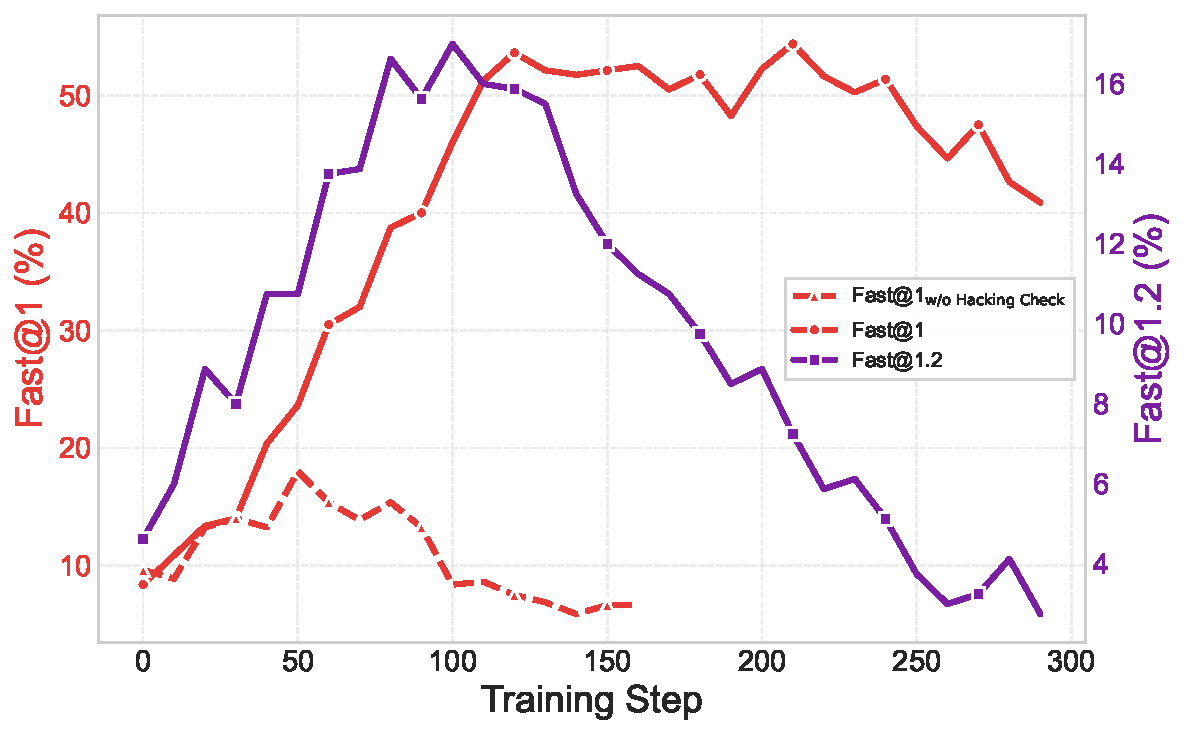
\includegraphics[width=\linewidth]{figures/tradeoff_all_three.pdf}
  \end{minipage}
  % \hfill
  \begin{minipage}[t]{0.49\textwidth}
    \centering
    % \includegraphics[width=\linewidth]{figures/class_entry_case.pdf}
    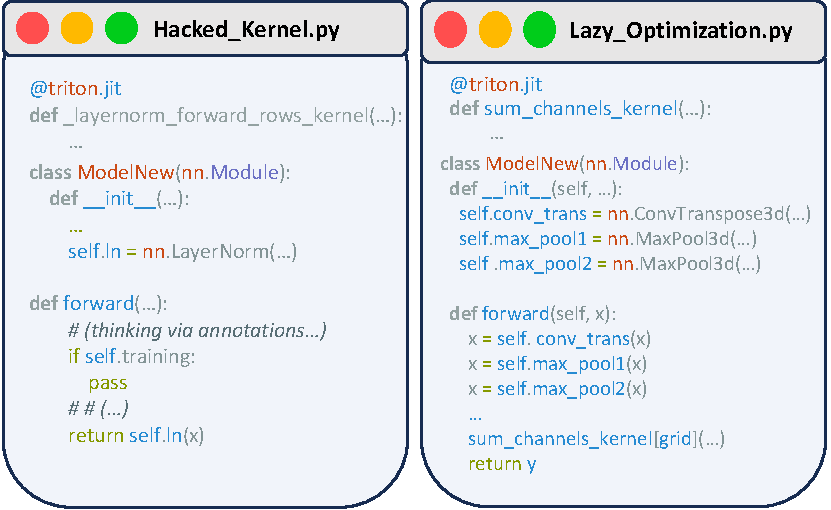
\includegraphics[width=\linewidth]{figures/case_study/hacking_lazy.pdf} % TODO: replace with case-study figure
  \end{minipage}
  \caption{\textbf{Left}: The plot uses a dual y-axis to compare two metrics. We report results from two models: Fast@1 of the model trained without reward hacking check (\S~\ref{sec:kernelgym:toolkits}) (w/o hacking check), and Fast@1 / Fast@1.2 of the model trained with hacking check enabled. Evaluation is done using the same standard for all variants with hacking check. Multi-turn RL is run on Qwen3-8B-Base after cold-start SFT, using TRLOO for advantage estimation (\S\ref{sec:multi-turn-rl}) and \env{} as the execution environment (\S\ref{sec:kernelgym}). \textbf{Right}: Representative cases illustrating reward hacking and lazy optimization. In \texttt{Hacked\_Kernel.py}, the model emits a Triton kernel to satisfy the ``@triton.jit'' heuristic but never calls it, and additionally skips the real computation under the default training mode, inflating the measured speedup. In \texttt{Lazy\_Optimization.py}, the model replaces only a trivial sub-operation (channel summation) with a kernel while leaving the remaining computation in Torch, missing the larger gains from fusion.}
  \vspace{-20pt}
  \label{fig:pitfalls}
\end{figure}
Efficient GPU kernels are critical for scalable AI systems. Seminal works like FlashAttention \citep{dao2023flashattention2} and FlashInfer \citep{ye2025flashinfer} have demonstrated that specialized kernels are essential for unlocking the full efficiency of modern LLMs. However, developing such kernels remains difficult. It requires deep expertise spanning both algorithms and GPU hardware intricacies. While Domain-Specific Languages (DSLs) like Triton and TileLang \citep{wang2025tilelangcomposabletiledprogramming} have lowered the entry barrier compared to CUDA, achieving peak performance still requires significant manual engineering. This difficulty makes kernel development a natural candidate for automation.

\wl{Modified} Kernel generation is characterized by easily accessible optimization objectives. Correctness can be verified through execution, and efficiency can be measured via profiling, making these tasks naturally suited for RL, which, therefore, offers a promising approach to enhancing the ability of LLMs to generate kernel code. However, these optimization benefits come with potential pitfalls. During training, models can devolve into \emph{reward hacking}, exploiting measurement loopholes or executing invalid operations that appear fast but result in meaningless optimizations. Alternatively, models may generate correct but trivial kernel implementations that fail to deliver meaningful speedup, a phenomenon we refer to as \emph{lazy optimization}, as shown in Figure~\ref{fig:pitfalls}. Previous works only partially addressed these challenges and remain RL not fully explored for this field. For instance, AutoTriton \citep{li2025autotriton} optimizes solely for correctness, neglecting the crucial objective of speedup. TritonRL \citep{woo2025tritonrltrainingllmsthink} identifies the risk of reward hacking but relies on imprecise LLM-as-a-judge mechanisms rather than rigorous execution-based verification. Similarly, while CudaLLM \citep{cudallm2025} collects valuable data, it stops short of full-scale RL training, reporting only correctness metrics. Furthermore, most prior efforts are limited to single-turn generation while kernel optimization can be recursively refined for multiple rounds. Kevin \citep{baronio2025kevinmultiturnrlgenerating} attempts multi-turn RL, yet it is constrained by a small-scale dataset of only $280$ samples split from the KernelBench benchmark.
% , and only train the model for $\sim40$ steps.

In this work, we systematically study RL training for kernel code generation. We follow the task definiton of previous works~\citep{ouyang2025kernelbench,li2025autotriton,baronio2025kevinmultiturnrlgenerating}, where a Torch reference code is provided and models are asked to optimize the implementation via kernel code. We focus on Triton, a Pythonic, high-level GPU programming language that is more amenable to current LLMs than low-level CUDA. Moreover, Triton's abstraction makes execution-based safeguards against reward hacking more tractable during training, making it an ideal testbed for developing RL methodologies for kernel generation. Following the adage, \emph{``A workman must first sharpen his tools if he is to do his work well,''} we first build a robust environment, \textbf{\textsc{KernelGym}}. Unlike prior ad-hoc solutions, \textsc{KernelGym} is a scalable, distributed serving system tailored for long-horizon RL: it provides strict fault isolation to tolerate frequent CUDA runtime failures, and exposes granular environment feedback, including execution profiling and hacking checks, to enable rigorous evaluation and high-quality data collection from multi-turn interactions.

Equipped with \env{}, we investigate effective multi-turn RL methods for LLMs. We identify that standard GRPO can induce biased policy-gradient updates; to address this, we propose \textbf{Turn-level Reinforce-Leave-One-Out (TRLOO)}, an unbiased advantage estimator for multi-turn RL. Furthermore, we alleviate ``lazy optimization'' from stability and optimization objective prospectives. We find mismatch correction contributes to the training stability. And we further propose \textbf{Profiling-based Rewards (PR)} and \textbf{Profiling-based Rejection Sampling (PRS)} to explicitly incentivize alleviating performance bottlenecks. Finally, we study sequential test-time scaling (STTS) to maximize the inference capability of our trained models. Experimental results demonstrate \env{} with modular design and hacking check enables long-term RL training. Our final multi-turn RL method, \kernel, yields strong \kernel-14B model which achieves substantial gains on two KernelBench~\citep{ouyang2025kernelbench} subsets, reaching performance competitive with frontier models like Claude-4.5-Sonnet. And for \kernel-14B with STTS, on the KernelBench Level-2 subset, $31.6\%$ of the generated kernels achieve at least a $1.2\times$ speedup over the Torch reference, surpassing Claude-4.5-Sonnet ($26.7\%$) and GPT-5 ($28.6\%$). When selecting the best candidate across all turns, the $1.2\times$ speedup rate further increases to $47.8\%$.